\documentclass[11pt]{article}


%%% Packages
%%
\usepackage{amsmath}
\usepackage{amsfonts}
\usepackage{amssymb}
\usepackage{fancyhdr}
\usepackage{float}
\usepackage{graphicx}
\usepackage[margin = 1 in, headheight = 13.6pt]{geometry}
\usepackage[linktoc=all]{hyperref}
\usepackage{listings}
\lstset{breaklines=true}
%%
%%%


%%% Formatting
%%
\parindent 0em
\parskip 1em
\pagestyle{fancy}
\fancyhead{}
\fancyfoot{}
\fancyhead[L]{\slshape\MakeUppercase{{\myTitle}}}
\fancyhead[R]{\slshape{\myName}}
\fancyfoot[C]{\thepage}
%%
%%%


%%% User defined variables
%%
\def \myTitle {ECE 404 Homework 2}
\def \myName {Elias Talcott}
\def \myDate {January 30, 2020}
%%
%%%


\begin{document}

\begin{titlepage}
\title{\myTitle}
\author{\myName}
\date{\myDate}
\maketitle
\vspace{1in}
\tableofcontents
\thispagestyle{empty}
\end{titlepage}

\section{Problem 1}
\subsection{Python Code}
\lstinputlisting[language = Python]{DES_text.py}
\pagebreak

\subsection{Encrypted and Decrypted Output}
\textbf{Encrypted Text}
\begin{figure}[h!]
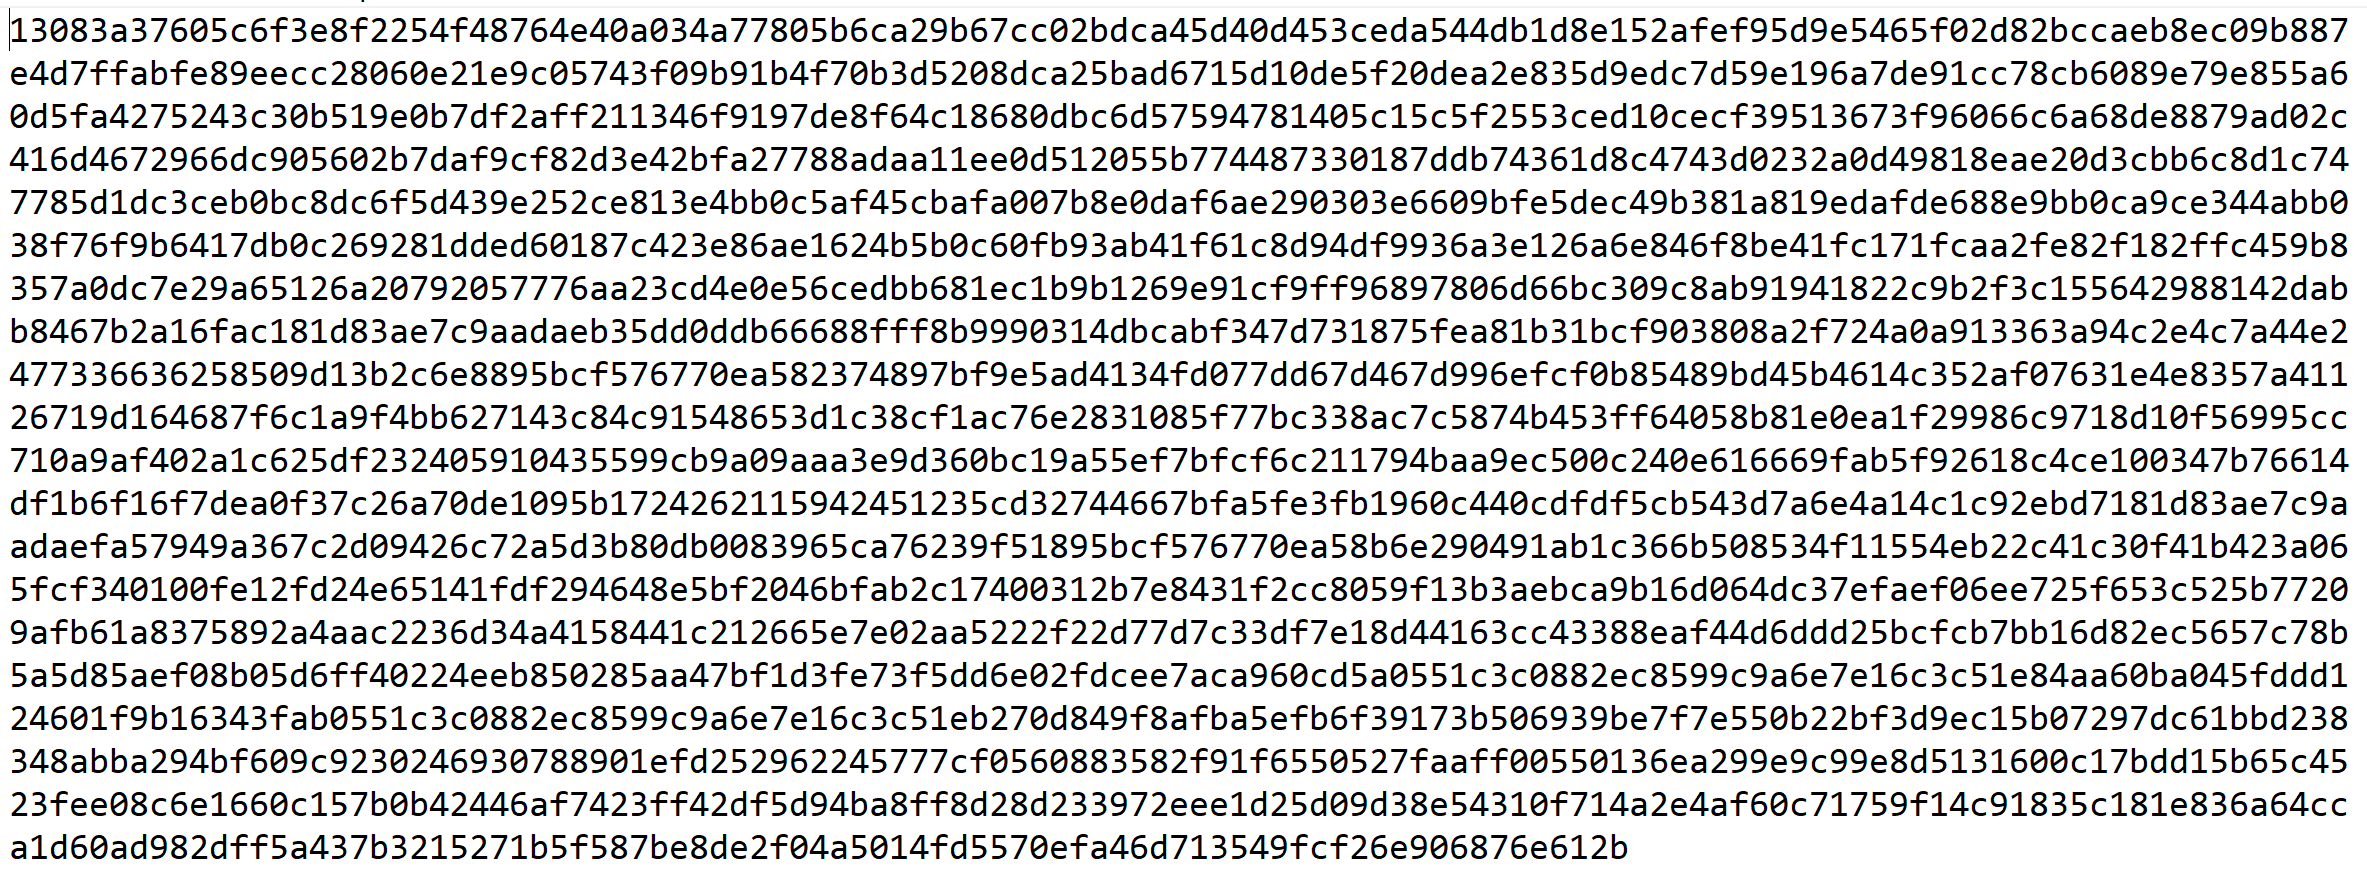
\includegraphics[width = \linewidth]{encrypted.png}
\end{figure}

\textbf{Decrypted Text}
\begin{figure}[h!]
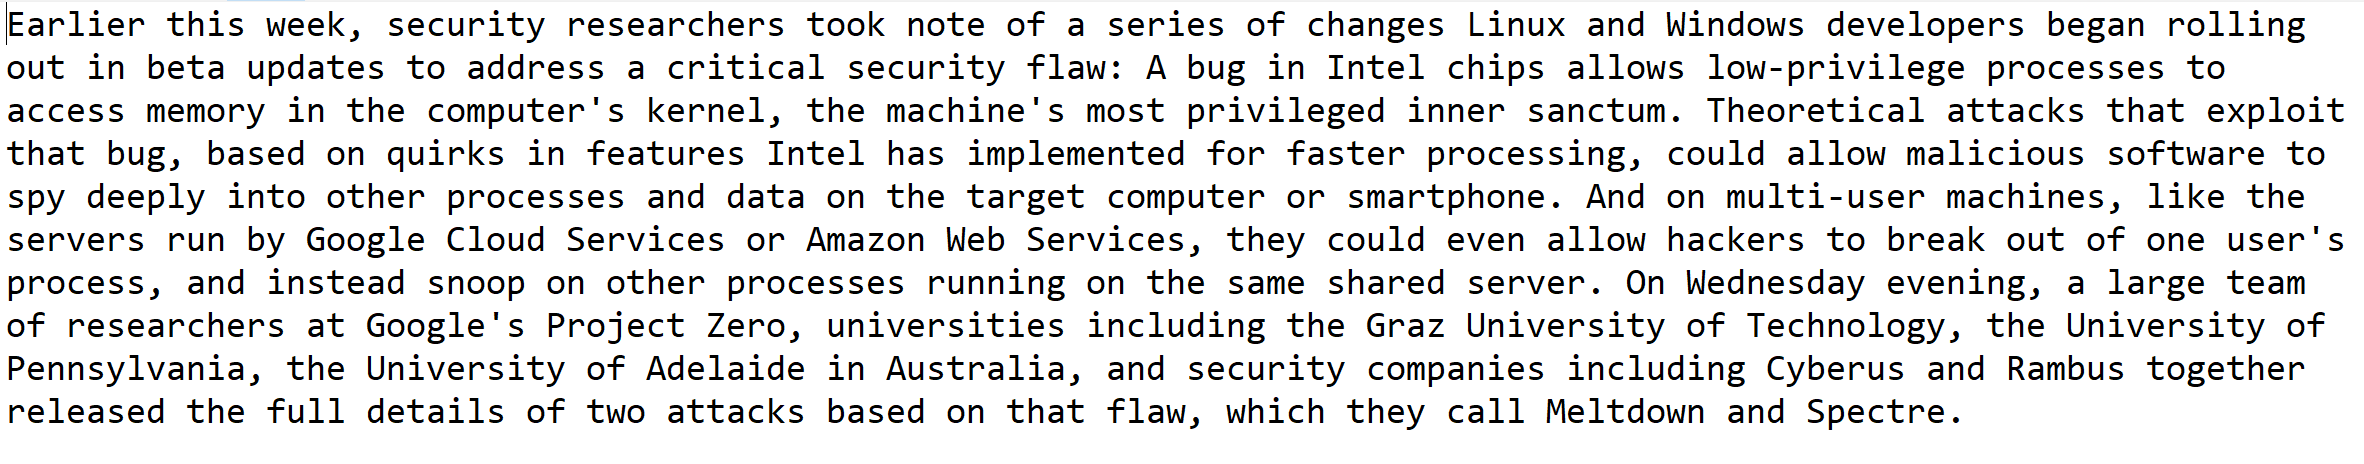
\includegraphics[width = \linewidth]{decrypted.png}
\end{figure}
\pagebreak

\subsection{Code Explanation}
In order to perform DES encryption, 16 rounds of the Feistel structure were used. First, the text file was read and checked to make sure it had a multiple of 64 bits. If not, 0s were added to pad the file. Then the file was split into blocks and encrypted one at a time. Each block was split in half, sent through 16 rounds, and then added to the ciphertext bitvector. Once all blocks had been encrypted, the ciphertext was written to the output file.

For decryption, the process was much the same. However, instead of splitting into left and right halves, the blocks were split into right and left halves. The order of the round keys was reversed, and the output blocks were also reversed when being added to the plaintext output.

\pagebreak

\section{Problem 2}
\subsection{Python Code}
\lstinputlisting[language = Python]{DES_image.py}
\pagebreak

\subsection{Original and Encrypted Output}
\textbf{Original Image}
\begin{figure}[h!]
	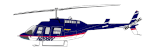
\includegraphics[scale=2]{OriginalImage.png}
\end{figure}

\textbf{Encrypted Image}
\begin{figure}[h!]
	
\includegraphics[scale=2]{EncryptedImage.png}
\end{figure}
\pagebreak

\subsection{Code Explanation}
In order to encrypt PPM files, the header had to be removed before starting DES encryption. This was done by reading the entire file and then splitting into 2 parts once 3 line returns had been detected. The header was written directly back to the encrypted file and the image data was encrypted normally. Since there were ASCII character 0-255 included, the utf-8 encoding was used to write to the encrypted file.

\end{document}